\newpage

\section{Instrukcja stworzenia klastra Kubernetes}\label{sec:instrukcja-stworzenia-klastra-kubernetes}

Ten załącznik stanowi instrukcję stworzenia klastra Kubernetes w chmurze obliczeniowej Oracle Cloud Infrastructure (OCI).
Klaster składa się z czterech węzłów, każdy z nich posiada 1 procesor (Oracle CPU, OCPU) oraz 6 GB pamięci RAM\@.
Zaproponowana infrastruktura obejmuje cztery maszyny wirtualne (c1, c2, c3, c4), load balancer (k8s) oraz sieć wirtualną (subnet-20230313-1902).
Uproszczony i uporządkowany model infrastruktury przedstawiono na rysunku~\ref{fig:infrastructure}.
Wszystkie wymienione elementy zostały wdrożone w ramach darmowego planu \emph{Always Free}.

Wykorzystanie czterech węzłów wraz z load balancerem, oraz odpowiednia konfiguracja, pozwala na zapewnienie wysokiej dostępności (ang. \emph{high availability}).

\begin{figure}[H]
    \centering
    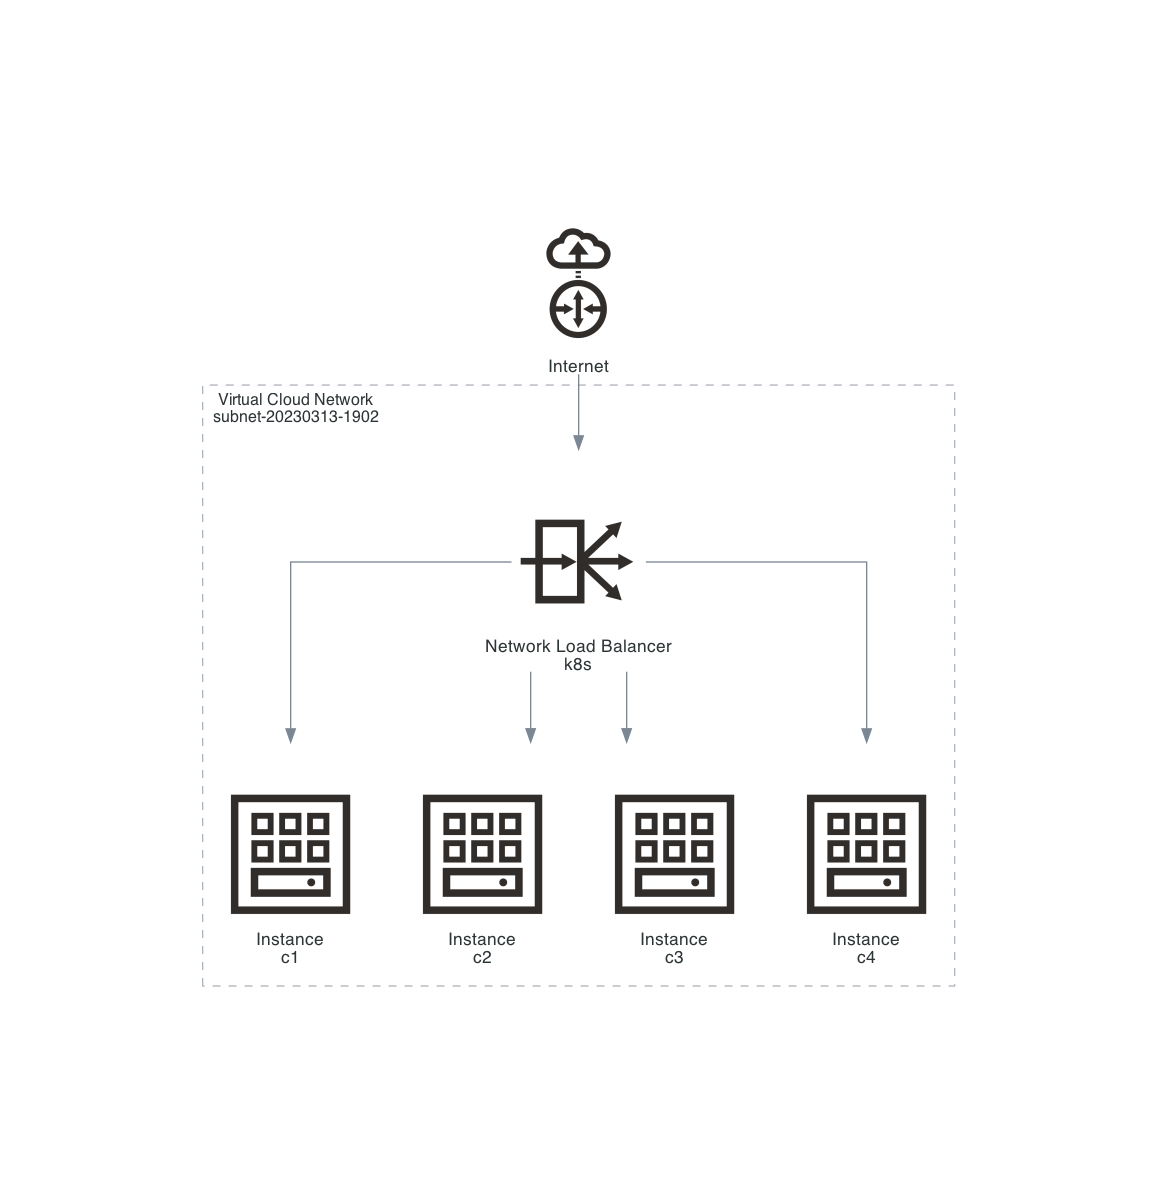
\includegraphics[width=\textwidth]{img/oci-infrastructure}
    \caption{Zaprojektowana infrastruktura}
    \label{fig:infrastructure}
\end{figure}

\subsection{Maszyny wirtualne}

Każdy węzeł klastra został uruchomiony na oddzielnej maszynie wirtualnej (ang. \emph{virtual machine, VM}).
Wszystkie węzły, w formie tabelki, przedstawiono na rysunku~\ref{fig:oci-compute-instances}.

\begin{figure}[H]
    \centering
    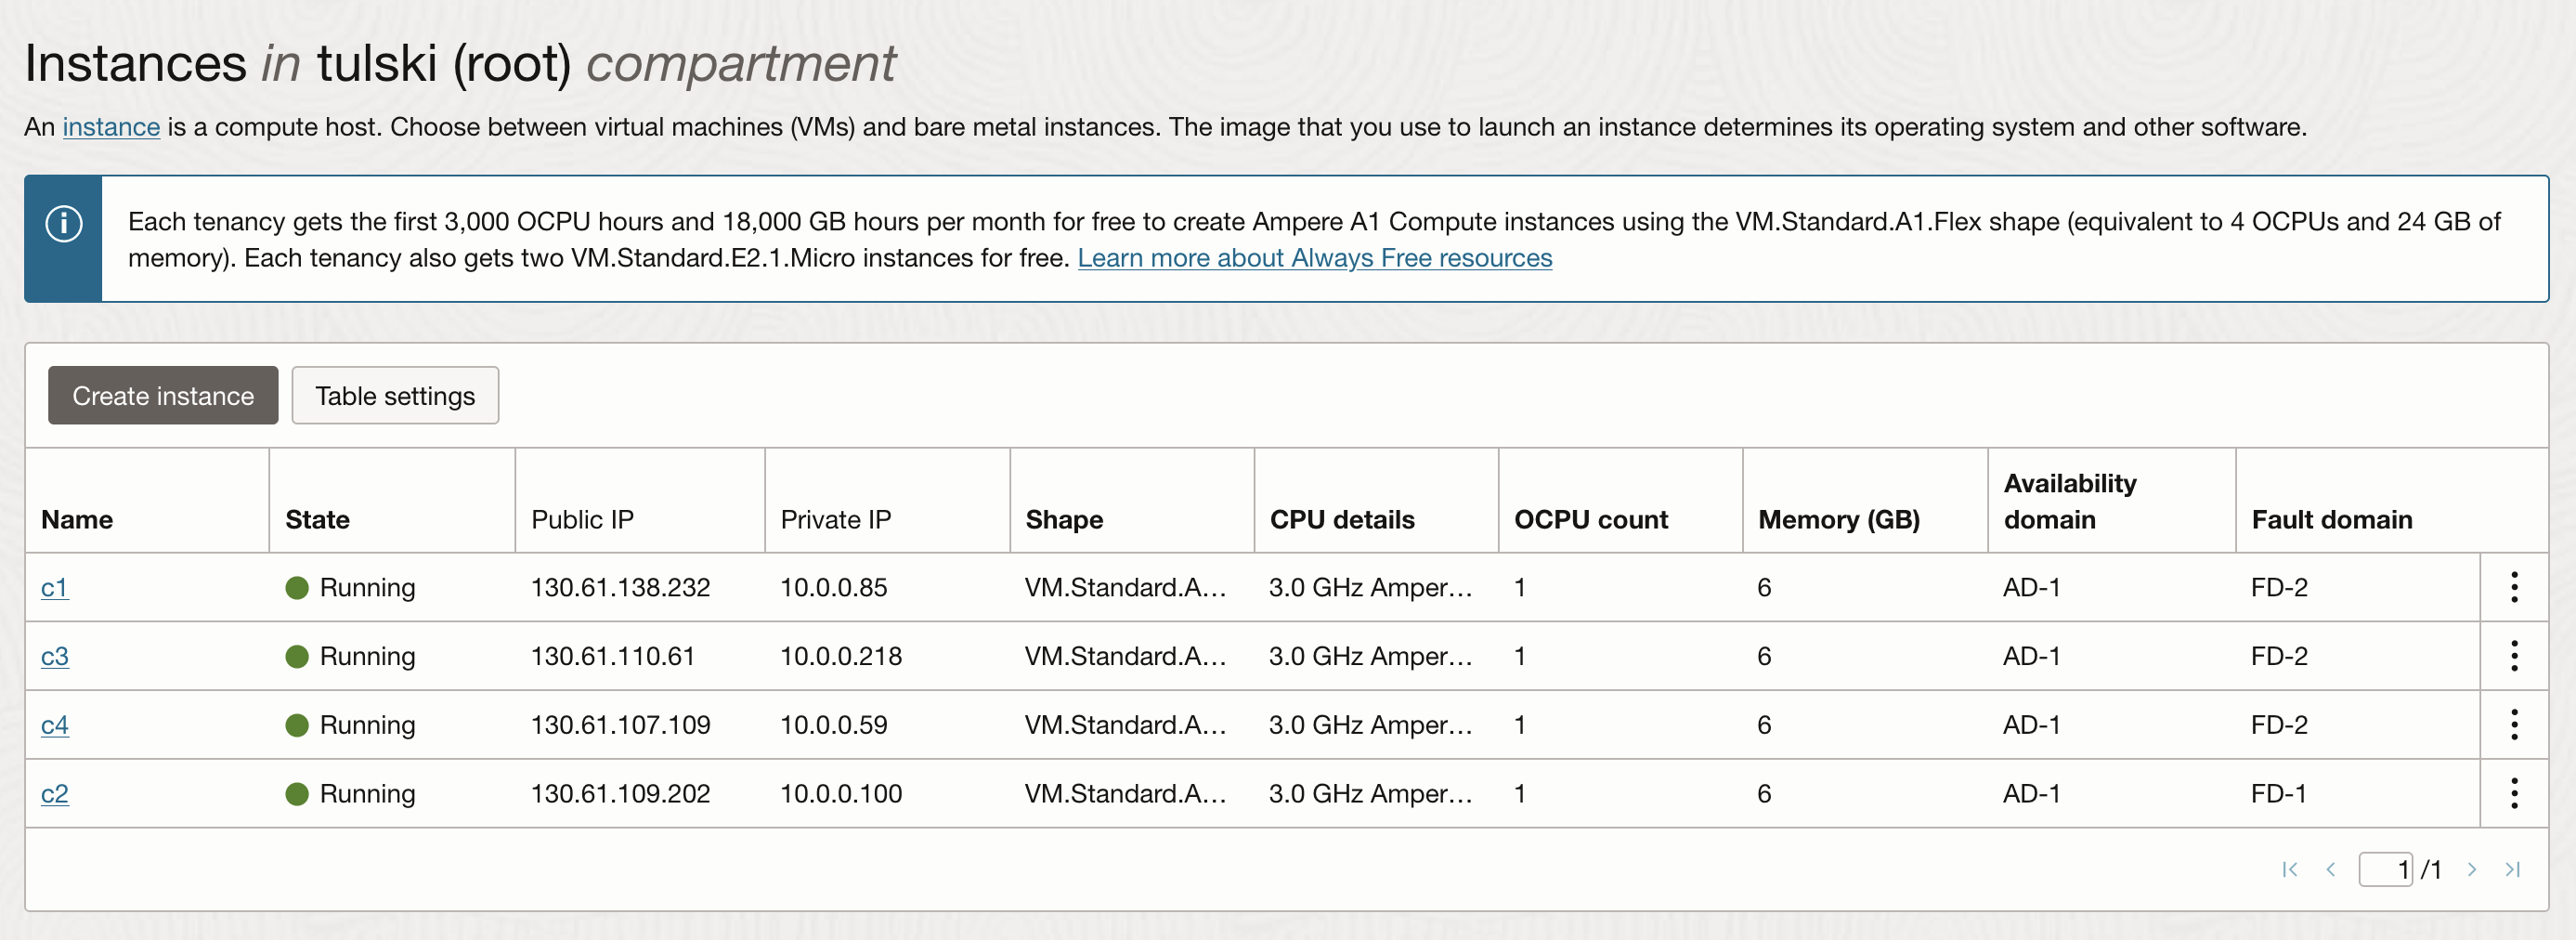
\includegraphics[width=\textwidth]{img/oci-compute-instances}
    \caption{Lista wszystkich maszyn wirtualnych}
    \label{fig:oci-compute-instances}
\end{figure}

\noindent Specyfikacja każdej z maszyn wirtualnych:
\begin{itemize}
    \item Kształt: VM.Standard.A1.Flex (Procesor Arm od Ampere)
    \item Liczba OCPU: 1
    \item Przepustowość sieci: 1 Gbps
    \item Pamięć RAM: 6 GB
    \item Obraz: Canonical Ubuntu 22.04 aarch64 2023.02.15-0
\end{itemize}

\noindent Szczegółową specyfikację jednej z maszyn wirtualnych przedstawiono na rysunku~\ref{fig:oci-instance-details}.

\begin{figure}[H]
    \centering
    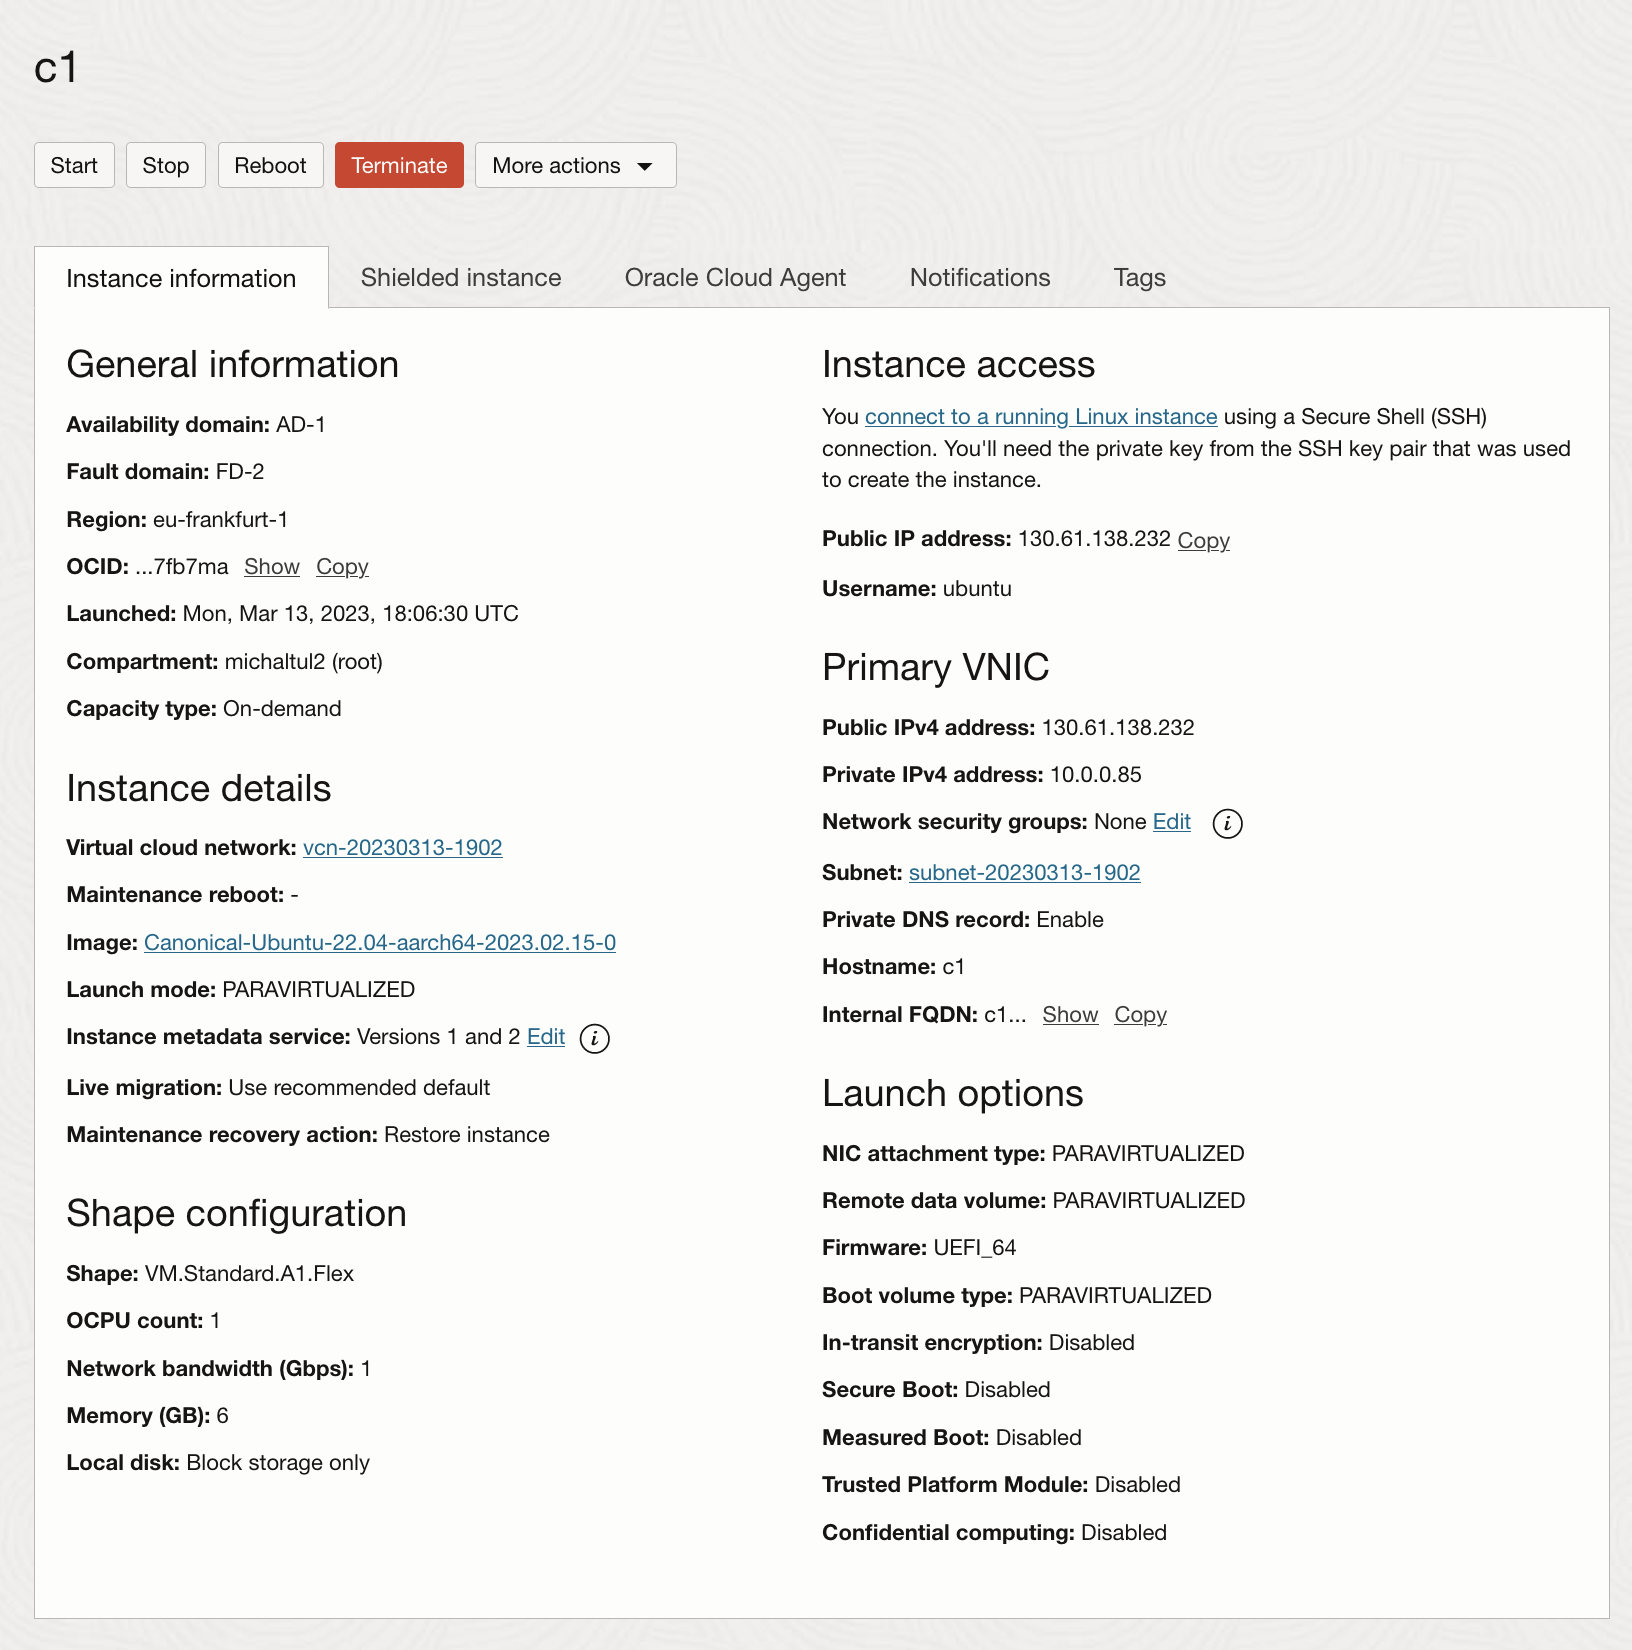
\includegraphics[width=\textwidth]{img/oci-instance-details}
    \caption{Specyfikacja maszyny wirtualnej c1}
    \label{fig:oci-instance-details}
\end{figure}

\subsection{Konfiguracja podsieci}

Wszystkie zasoby znajdują się w jednej wirtualnej podsieci (ang. \emph{virtual cloud network}, VCN) subnet-20230313-1902, która stanowi bezpieczne i izolowane środowisko sieciowe.
Informacje o podsieci przedstawiono na rysunku~\ref{fig:oci-subnet}.

\begin{figure}[H]
    \centering
    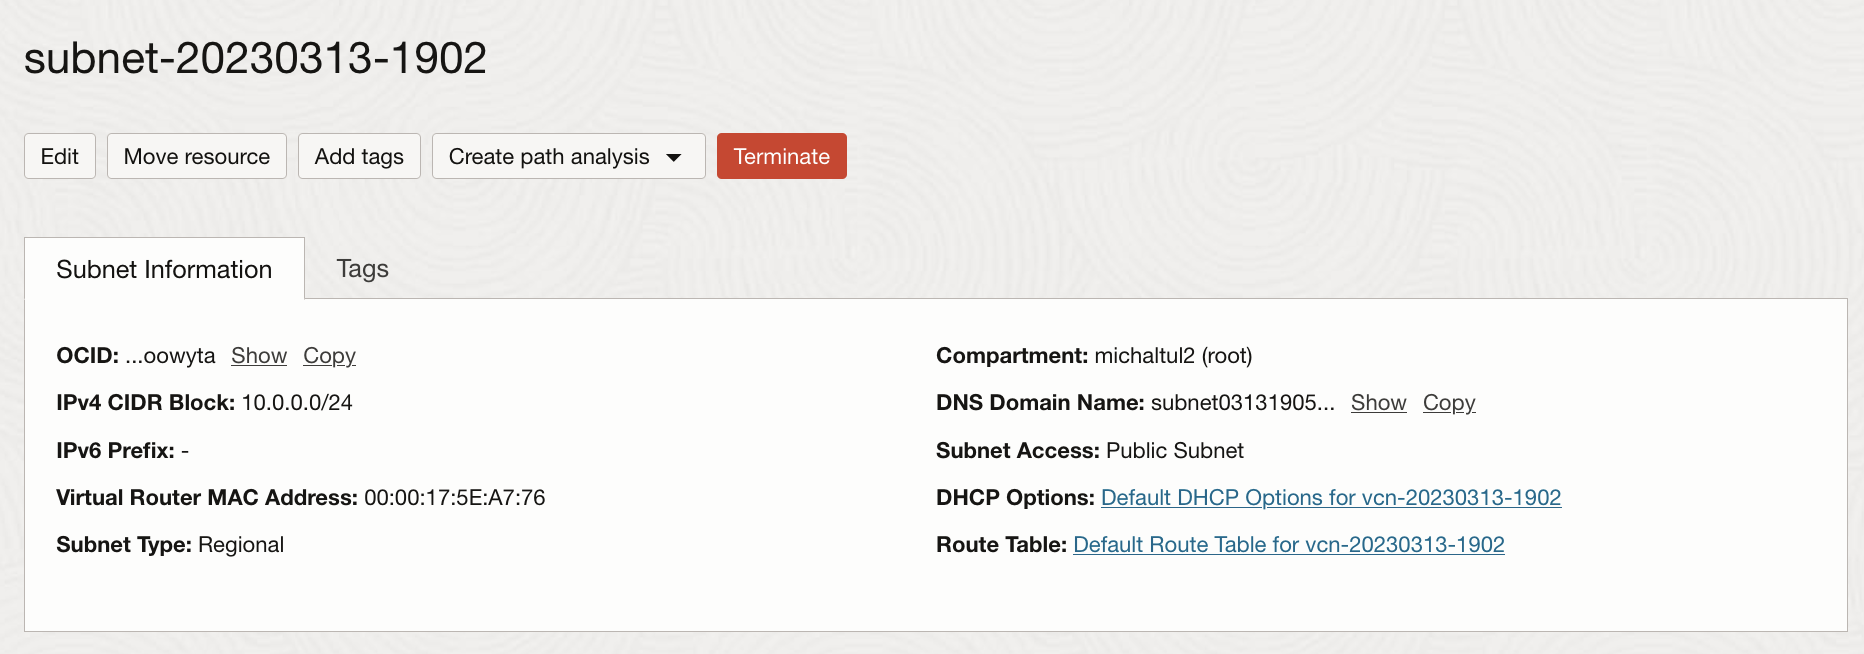
\includegraphics[width=\textwidth]{img/oci-subnet}
    \caption{Podsieć subnet-20230313-1902}
    \label{fig:oci-subnet}
\end{figure}

\noindent Domyślne reguły VCN\cite{oci-security-lists} pozwalają na:
\begin{enumerate}
    \item ruch TCP na porcie usługi SSH (22) z autoryzowanych adresów IP\@,
    \item ruch ICMP typu 3 o kodzie 4 (ang. \emph{Fragmentation Needed and Don't Fragment was Set}) z dowolnego adresu IP,
    \item ruch ICMP typu 3 z wszystkich hostów znajdujących się w danej podsieci,
    \item ruch wychodzący.
\end{enumerate}

\noindent Aby wykorzystać klaster jako platformę wdrożeniową dla aplikacji internetowych, konieczne jest dodanie dwóch dodatkowych reguł.

\begin{enumerate}
    \item Reguła pozwalająca na ruch TCP z dowolnego źródła na porty 80 i 443.
    \item Reguła pozwalająca na cały ruch z adresu IP administratora - wymagana do zdalnego zarządzania klastrem przez Kubernetes API (kubectl).
\end{enumerate}

\noindent Kompletna lista wszystkich reguł sieciowych dla stworzonej podsieci subnet-20230313-1902 została zaprezentowana na rysunku~\ref{fig:oci-subnet-ingress-rules}.

\begin{figure}[H]
    \centering
    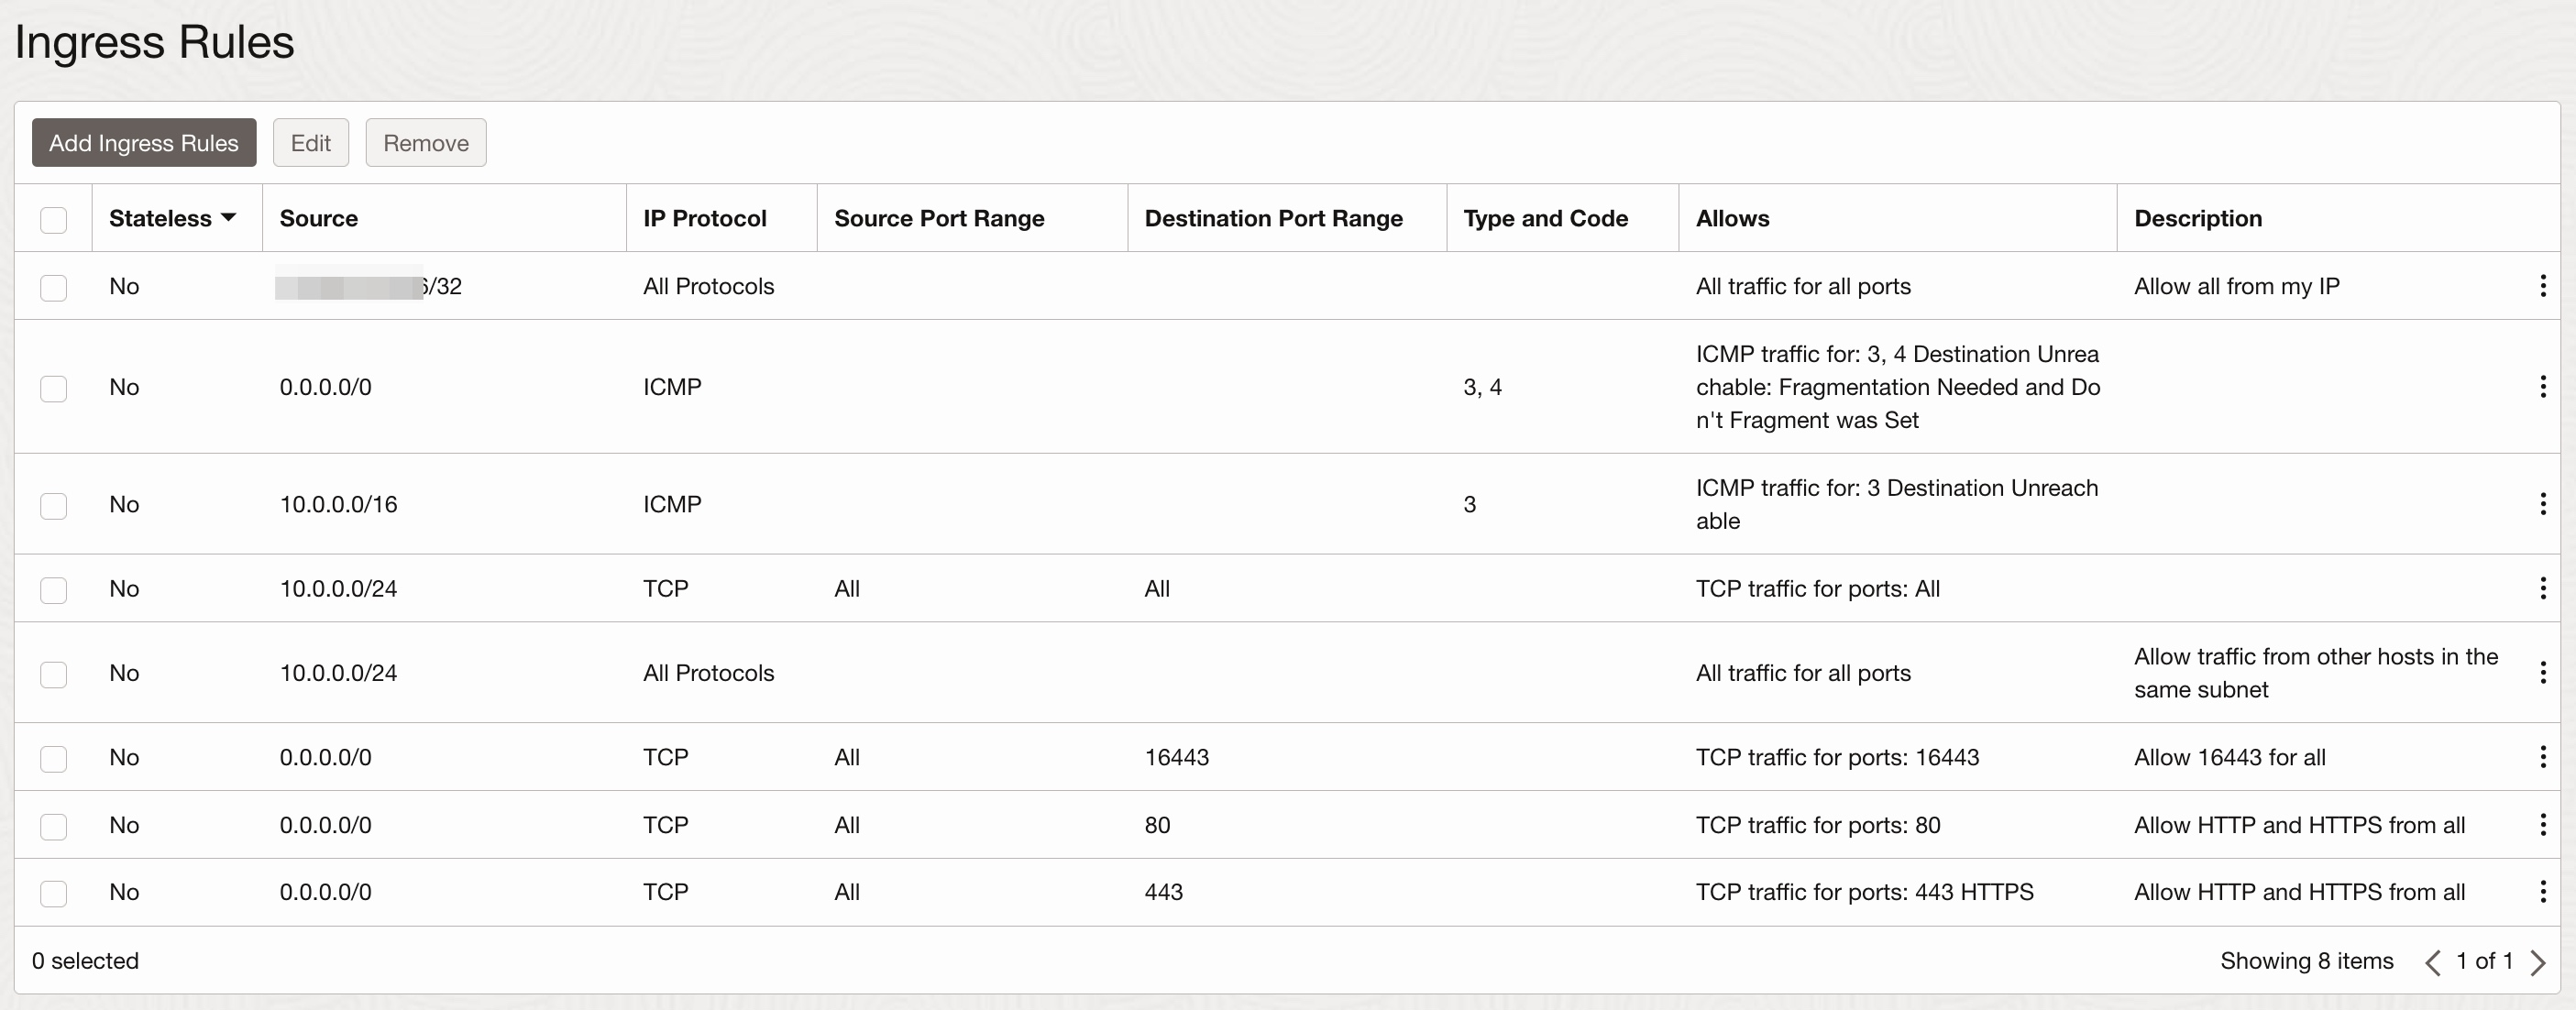
\includegraphics[width=\textwidth]{img/oci-subnet-ingress-rules}
    \caption{Reguły dla ruchu przychodzącego}
    \label{fig:oci-subnet-ingress-rules}
\end{figure}

Zmiany na poziome usług sieciowych OCI są niewystarczające, ponieważ ruch zostanie zablokowany przez domyślne reguły firewalla systemowego maszyn wirtualnych.
Aby osiągnąć oczekiwany rezultat konieczna jest modyfikacja pliku \texttt{/etc/iptables/rules.v4} na każdej z maszyn wirtualnych.

\noindent Należy dodać dwie reguły:

\begin{enumerate}
    \item Reguła zezwalająca na ruch wejściowy pochodzący z publicznego adresu IP administratora.\\
    \mintinline{text}{-I INPUT -s ADMIN_PUBLIC_IP/32 -j ACCEPT}
    \item Reguła pozwalająca na ruch przychodzący z dowolnego adresu w podsieci.\\
    \mintinline{text}{-I INPUT -s 10.0.0.0/24 -j ACCEPT}
\end{enumerate}

\noindent Dodatkowo, konieczne jest usunięcie wpisu, który blokuje wiadomości ICMP (ping):\\
\mintinline{text}{-A FORWARD -j REJECT --reject-with icmp-host-prohibited}

\subsection{Network Load Balancer}

Load Balancer (LB) to technologia, która, podobnie do reverse proxy, ma na celu kierowanie żądań użytkowników do odpowiednich serwerów.
Każdy LB implementuje pewien zestaw reguł i algorytmów, który równomiernie rozkładają ruch na wszystkie serwery w grupie mogące go obsłużyć, tak aby sprostować aktualnemu obciążeniowi.
Dzięki temu zapewnia pryncypium wysokiej dostępności (high availability), niezawodności i skalowalność systemu.
W związku z tym, że Load Balancer ciągle monitoruje aktywność węzłów, jest w stanie szybko wykryć ewentualną awarię i automatycznie przekierować ruch do pozostałych, sprawnych węzłów.
Prostą analogią dla Load Balancera jest policjant stojący na skrzyżowaniu.

Dodatkową zaletą LB jest uproszczenie konfiguracji DNS - wystarczy dodanie jednego rekord typu A z publicznym adresem IP wskazującym na LB\@.
Eliminuje to potrzebę tworzenia osobnych wpisów dla każdego węzła, co komplikowałoby konfigurację i utrudniałoby jej utrzymanie.

Z powodu zapewnienia wysokiej dostępności, równomiernego rozłożenia ruchu, skalowalności i uproszczeniu konfiguracji DNS, jak i wielu innych niewspomnianych korzyści, LB jest kluczowym elementem wielu rozbudowanych systemów.

Jednym z rodzajów Load Balancera jest Network Load Balancer (NLB), który działa na warstwie 3 i 4 modelu OSI wykorzystując protokoły TCP, UDP i ICMP\@.
NLB przekazuje pakiety do i z serwera nadrzędnego na podstawie informacji na poziomie IP, portu i protokołu bez sprawdzania pakietów.

Utworzony Network Load Balancer k8s znajduje się w wcześniej stworzonej podsieci subnet-20230313-1902.

\autoref{fig:oci-network-load-balancer-k8s} przedstawia informacje o wdrożonym NLB k8s.

\begin{figure}[H]
    \centering
    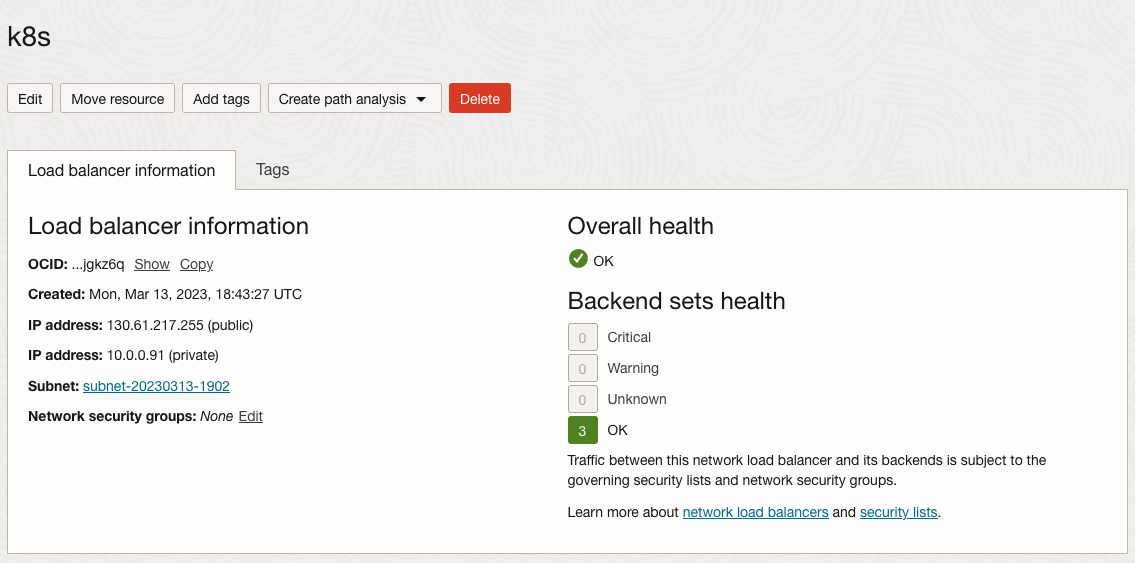
\includegraphics[width=\textwidth]{img/oci-network-load-balancer-k8s}
    \caption{Informacje o NLB k8s}
    \label{fig:oci-network-load-balancer-k8s}
\end{figure}

NLB k8s został skonfigurowany tak aby działał dla ruchu HTTP (port 80), HTTPS (port 443) oraz Kubernetes API (port 16443).
Dla każdego z rodzajów ruchu został utworzony Backend Set (zob. \autoref{fig:oci-network-load-balancer-k8s-backend-sets}) oraz Listener (zob. \autoref{fig:oci-network-load-balancer-k8s-listeners}).

\begin{figure}[H]
    \centering
    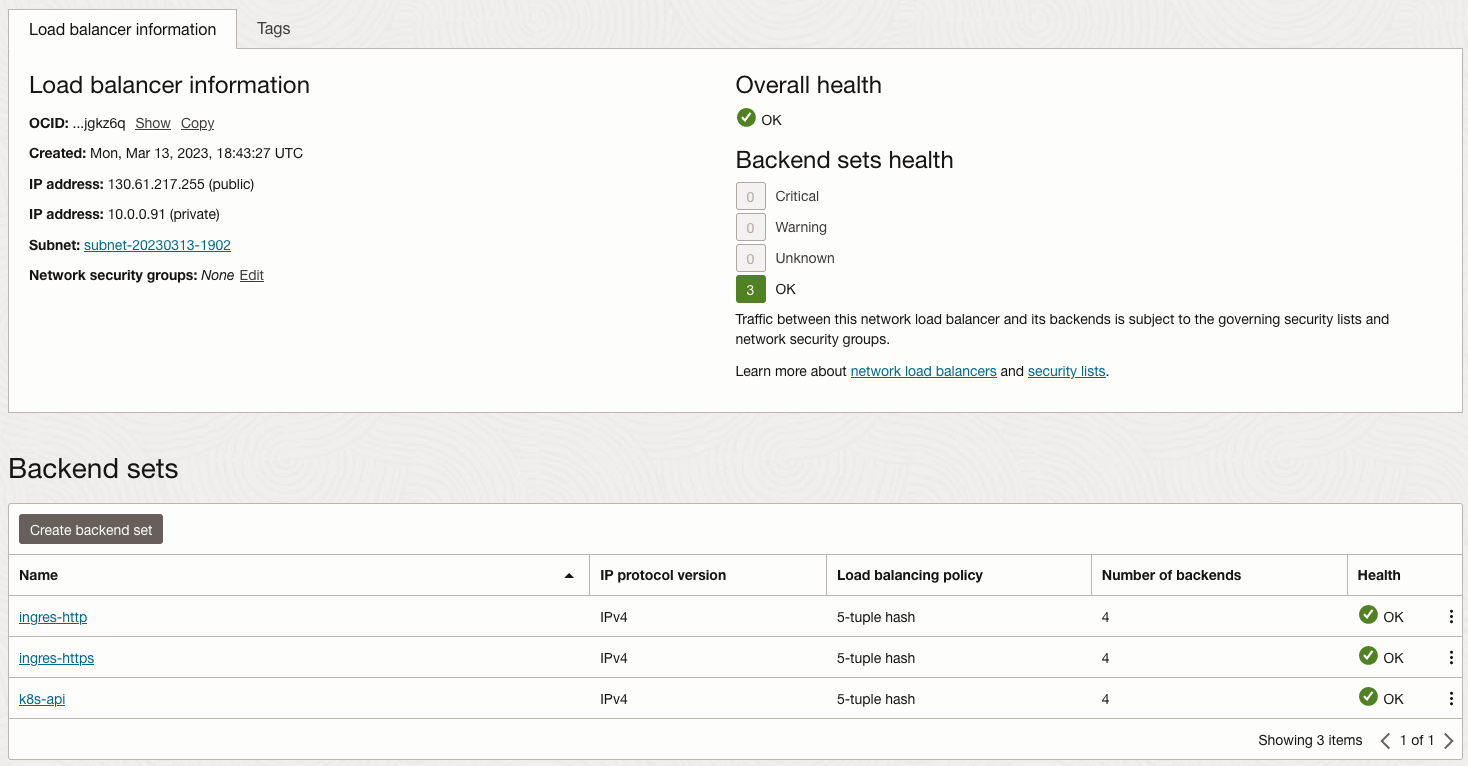
\includegraphics[width=\textwidth]{img/oci-network-load-balancer-k8s-backend-sets}
    \caption{Backend Sets stworzonego Network Load Balancera k8s}
    \label{fig:oci-network-load-balancer-k8s-backend-sets}
\end{figure}

\begin{figure}[H]
    \centering
    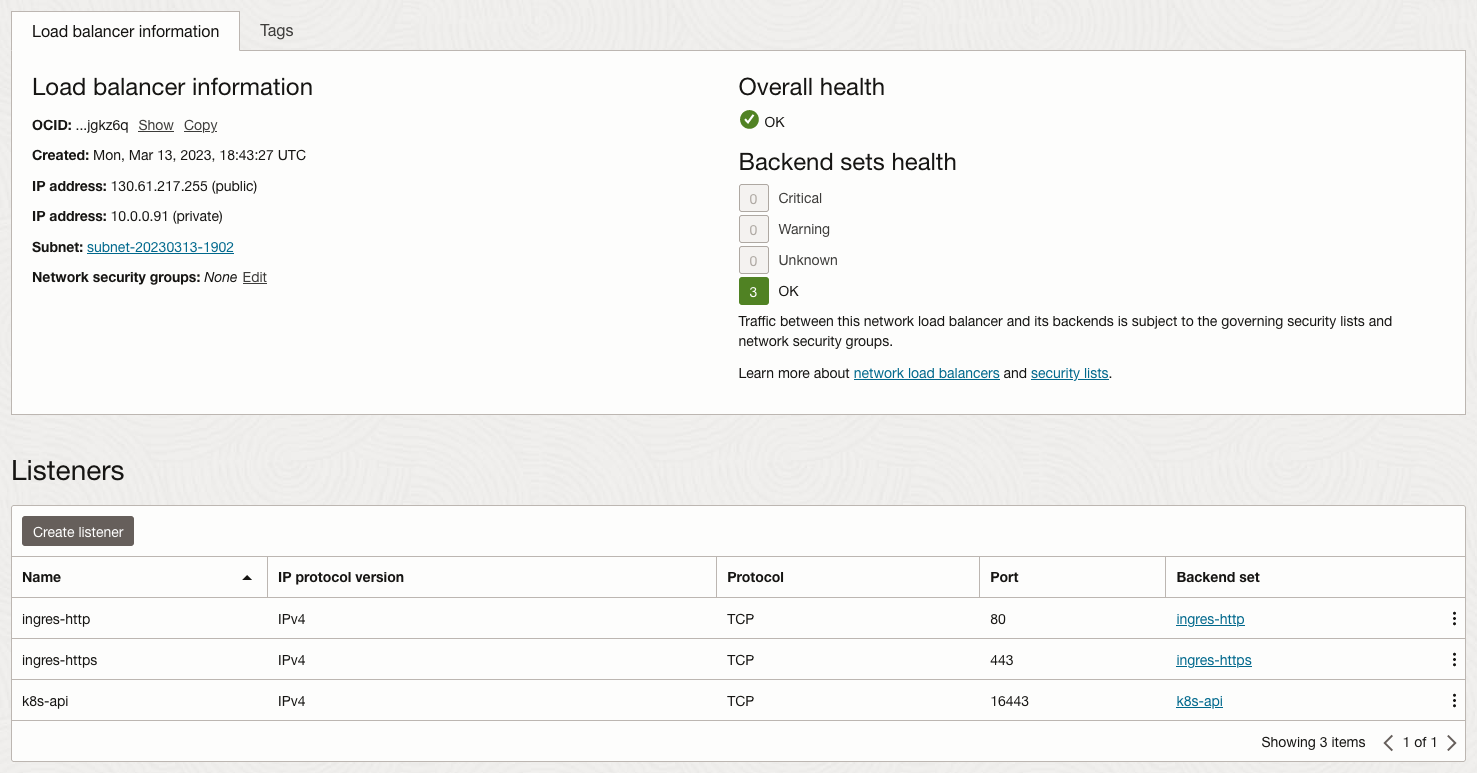
\includegraphics[width=\textwidth]{img/oci-network-load-balancer-k8s-listeners}
    \caption{Listeners stworzonego Network Load Balancera k8s}
    \label{fig:oci-network-load-balancer-k8s-listeners}
\end{figure}

Load Balancer regularnie monitoruje aktywność każdego węzła za pomocą zdefiniowanego testu Health Check.
Dla pierwszych dwóch Backend Sets - \texttt{ingress-http} (zob. \autoref{fig:oci-network-load-balancer-ingress-http-health-check}) oraz \texttt{ingress-https} (zob. \autoref{fig:oci-network-load-balancer-ingress-https-health-check})- test polega na wysłaniu zapytania z użyciem kolejno protokołu HTTP i HTTPS na ścieżkę \url{/}.
Oczekiwaną odpowiedzią serwera jest status 404.

\begin{multicols}{2}
    \begin{figure}[H]
        \centering
        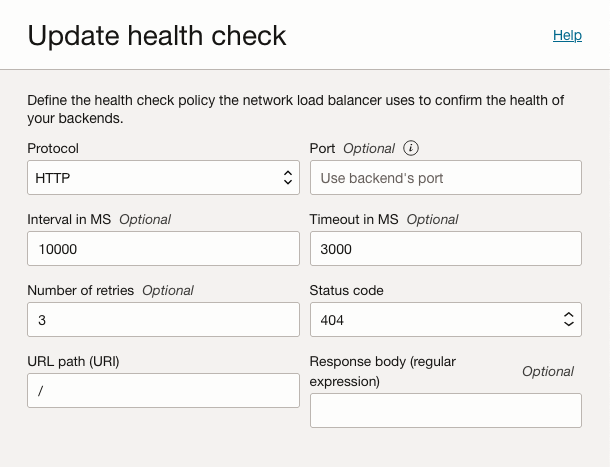
\includegraphics[width=0.5\textwidth]{img/oci-network-load-balancer-ingress-http-health-check}
        \caption{Health Check dla ingress-http}
        \label{fig:oci-network-load-balancer-ingress-http-health-check}
    \end{figure}
    \begin{figure}[H]
        \centering
        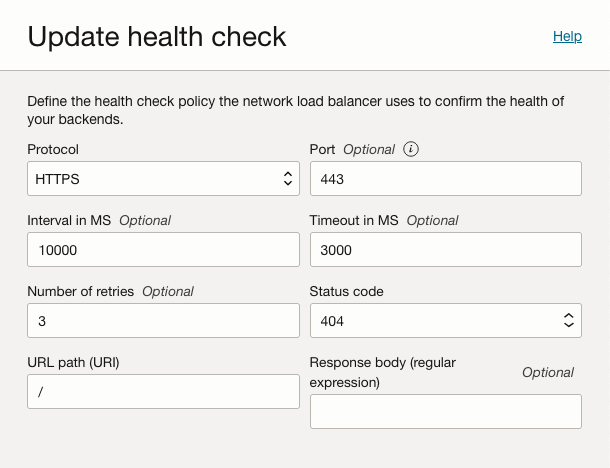
\includegraphics[width=0.5\textwidth]{img/oci-network-load-balancer-ingress-https-health-check}
        \caption{Health Check dla ingress-https}
        \label{fig:oci-network-load-balancer-ingress-https-health-check}
    \end{figure}
\end{multicols}

Ostatni Backend Set, czyli  k8s-api, polega na wysłaniu zapytania protokołem HTTPS na port 16443 do ścieżki \url{/healthz}, gdzie oczekiwaną odpowiedzią serwera jest status 200 (zob. \autoref{fig:oci-network-load-balancer-k8s-api-health-check}).
\begin{figure}[H]
    \centering
    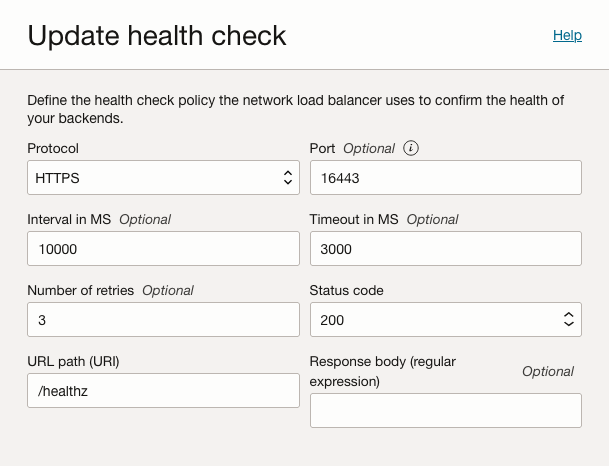
\includegraphics[width=0.7\textwidth]{img/oci-network-load-balancer-k8s-api-health-check}
    \caption{Health Check dla k8s-api}
    \label{fig:oci-network-load-balancer-k8s-api-health-check}
\end{figure}

\subsection{Instalacja Kubernetes}

Klaster wykorzystuje dystrybucję MicroK8s (zob. \autoref{subsec:microk8s}) w wersji 1.23.
Instalację MicroK8s przeprowadzono na każdej z maszyn wirtualnych poleceniem~\autoref{lst:microk8s-install}.

\begin{listing}[H]
    \begin{minted}[xleftmargin=10pt,linenos]{bash}
    apt update && \
        apt install docker.io -y && \
        snap install microk8s --classic --channel=1.23/stable
    \end{minted}
    \caption{Polecenie instalacyjne MicroK8s}
    \label{lst:microk8s-install}
\end{listing}

\subsection{Konfiguracja certyfikatów Kubernetes API}

Kubernetes API stanowi kluczowy element systemu z perspektywy cyberbezpieczeństwa.
Jednym z sposobów jego zabezpieczenia jest wymóg szyfrowanej komunikacji HTTPS, opartej na zweryfikowanym certyfikacie.
Domyślne generowane przez MicroK8s certyfikaty pozwalają na połączenia z lokalnych adresów IP (zwykle adresów LAN) oraz komunikację z adresami mDNS (komunikacja w obrębie klastra, z adresów takich jak kubernetes.default lub kubernetes.default.svc.cluster.local).
Aby umożliwić zdalne połączenie z Kubernetes API z internetu, niezbędna jest modyfikacja sekcji alt\_name pliku szablonu Certificate Signing Request (CSR) znajdującego się pod ścieżką \url{ /var/snap/microk8s/current/certs/csr.conf.template}.
Modyfikacja musi zostać wykonana na każdej z maszyn wirtualnych.

\noindent Modyfikacja polega na dodaniu do sekcji alt\_names:
\begin{enumerate}
    \item publicznego adresu IP maszyny wirtualnej,
    \item prywatnego adresu IP maszyny wirtualnej,
    \item publicznego adresu IP load balancera.
\end{enumerate}

\noindent\autoref{lst:domyslna-konfiguracja-alt-names} przedstawia domyślną, niezmienioną sekcję alt\_names.

\begin{listing}[H]
    \begin{minted}[xleftmargin=10pt,linenos]{text}
[ alt_names ]
DNS.1 = kubernetes
DNS.2 = kubernetes.default
DNS.3 = kubernetes.default.svc
DNS.4 = kubernetes.default.svc.cluster
DNS.5 = kubernetes.default.svc.cluster.local
IP.1 = 127.0.0.1
IP.2 = 10.152.183.1
    \end{minted}
    \caption{Domyślna sekcja alt\_names maszyny wirtualnej c1}
    \label{lst:domyslna-konfiguracja-alt-names}
\end{listing}

\noindent\autoref{lst:zmodyfikowana-konfiguracja-alt-names} przedstawia odpowiednio zmodyfikowaną sekcję alt\_names.

\begin{listing}[H]
    \begin{minted}[xleftmargin=10pt,linenos]{text}
[ alt_names ]
DNS.1 = kubernetes
DNS.2 = kubernetes.default
DNS.3 = kubernetes.default.svc
DNS.4 = kubernetes.default.svc.cluster
DNS.5 = kubernetes.default.svc.cluster.local
IP.1 = 127.0.0.1
IP.2 = 10.152.183.1
IP.100 = 130.61.138.232 # Publiczny adres IP maszyny wirtualnej
IP.110 = 10.0.0.85      # Prywanty adres IP maszyny wirtualnej
IP.120 = 130.61.217.255 # Publiczny adres IP load balancera
    \end{minted}
    \caption{Zmodyfikowana sekcja alt\_names na maszynie wirtualnej c1}
    \label{lst:zmodyfikowana-konfiguracja-alt-names}
\end{listing}

\noindent Po modyfikacji pliku konieczne jest uruchomienie polecenia odświeżającego certyfikaty MicroK8s (zob. \autoref{lst:polecenie-odswiezajace-certyfikaty}) i ponowne uruchomienie maszyny (reboot).

\begin{listing}[H]
    \begin{minted}[xleftmargin=10pt,linenos]{bash}
    sudo microk8s refresh-certs
    \end{minted}
    \caption{Polecenie odświeżające certyfikaty MicroK8s}
    \label{lst:polecenie-odswiezajace-certyfikaty}
\end{listing}

\subsection{Formowanie klastra Kubernetes}

\noindent Formowanie klastra w Kubernetes polega na zintegrowaniu węzłów uruchomionych na różnych maszynach wirtualnych, aby wspólnie tworzyły jednolity system.
Poniżej przedstawione są kroki niezbędne do uformowania klastra.

\begin{enumerate}
    \item Określ, która z maszyn wirtualnych będzie pełnić rolę głównego węzła (ang. \emph{master node}). To on będzie koordynować dodawanie kolejnych węzłów do klastra.
    \item Na wyznaczonym głównym węźle wykonaj polecenie \mintinline{bash}{microk8s add-node}.
          Wynikiem będzie polecenie do dołączenia do klastra mające postać:
    \begin{figure}[H]
        \begin{minted}[xleftmargin=10pt,linenos]{bash}
    microk8s join <vm_private_ip>:25000/<token>
        \end{minted}
        \label{fig:join-cluster-command}
    \end{figure}
    \item Wykonaj otrzymane w poprzednim kroku polecenie na każdej maszynie wirtualnej, która ma zostać częścią klastra, ale jeszcze w nim nie jest.
    \item Dla każdej kolejnej maszyny, która ma dołączyć do klastra, powtarzaj kroki 2 i 3.
\end{enumerate}